% Created 2017-04-18 mar. 11:39
\documentclass[10pt, aspectratio=169]{beamer}
\usepackage[english,whiteheader]{phimecapr}
\usepackage{fixltx2e}
\usepackage{graphicx}
\usepackage{longtable}
\usepackage{float}
\usepackage{wrapfig}
\usepackage{soul}
\usepackage{textcomp}
\usepackage{marvosym}
\usepackage{wasysym}
\usepackage{latexsym}
\usepackage{amssymb}
\usepackage{fancyvrb}
\usepackage{hyperref}
\tolerance1000
\providecommand{\alert}[1]{\textbf{#1}}

% fancy verbatim fontsize
\fvset{fontsize=\scriptsize}

\title{Creating a distributed python wrapper with otwrapy}
\subtitle{HPC and Uncertainty Treatment}
\author[G. Blondet]{Gaëtan Blondet, Phimeca Engineering}
\date[OtWraPy - May 11-13 2020]{PRACE Advanced Training Center, May 11-13 2020\\EDF – Phimeca – Airbus Group – IMACS – CEA}

\hypersetup{colorlinks=true, linkcolor=., urlcolor={orange}}

\begin{document}

\begin{frame}[plain]
  \titlepage
\end{frame}

\begin{frame}{\tableofcontentstitle}
  \tableofcontents[hideallsubsections]
\end{frame}

\label{sec-1}
\section{Introduction}

\begin{frame}
\frametitle{Introduction}
\begin{itemize}
\item What is a wrapper?
	\begin{itemize}
		\item a python interface with your external code.
		\item able to take advantage of multi-core computers and HPC clusters, to distribute multiple evaluations of your code.
  	\end{itemize}
  	
\item Presentation goal: Show you how to create a distributed wrapper to efficiently carry on uncertainty studies.

\item Based on the module \href{http://openturns.github.io/otwrapy/master/index.html}{otwrapy} available at \href{https://github.com/openturns/otwrapy}{GitHub}. Initially developed at \href{http://www.phimeca.com}{Phimeca engineering}.
\item A good working example can be found on the  \href{https://github.com/openturns/otwrapy/tree/master/otwrapy/examples/beam}{otwrapy repository example}.
\end{itemize}
\end{frame}


\begin{frame}[fragile]
\frametitle{What makes a good wrapper ?}
\begin{itemize}
\item It is distributed and avoids conflict between runs.
\item You can use it as a script (argsparse module):

\begin{Verbatim}[xleftmargin=10mm]
   >> python wrapper.py -X 170 3 0.05
\end{Verbatim}

\item It is able to run on different environments:
\begin{itemize}
\item Workstation
\item Office made heterogeneous clusters --> e.g. IPyparallel or dispy
\item HPC through submission scripts --> e.g. TGCC or Poincare
\item Cloud solutions --> e.g. Simulagora or DominoUp
\end{itemize}
\item It catches and logs errors for easy debugging.
\item It can either run or simply prepare runs --> useful when running on
  clusters.
\end{itemize}
All of this  might seem complex, but wrappers are repetitive and
\href{https://github.com/openturns/otwrapy}{otwrapy} is here for you !
\end{frame}


\section{Basic skeleton of a wrapper}
\label{sec-3}
\begin{frame}[fragile]
\frametitle{Basic skeleton of a wrapper}
\begin{itemize}
\item Assumption: you want to wrap an external code not written in Python.
\item An OpenTURNS wrapper is a subclass of \texttt{ot.OpenTURNSPythonFunction}
  for which at least the method \texttt{\_exec(X)} should be
  overloaded. Additionally, you can overload \texttt{\_exec\_sample(X)}, but
  with \href{http://openturns.github.io/otwrapy/master/_generated/otwrapy.Parallelizer.html}{otwrapy.Parallelizer()} there is no need to.
\item If your code handles the gradient and the hessian, you can
  respectively overload \texttt{\_gradient(X)} and \texttt{\_hessian(X)}.
\end{itemize}
\vfill
\begin{Verbatim}[xleftmargin=10mm]
class Wrapper(ot.OpenTURNSPythonFunction):
    """Wrapper of my external code.
    """
    def __init__(self):
        """Initialize the wrapper with 4 and 1 as input and output dimension.
        """
        super(Wrapper, self).__init__(4, 1)
        # Do other stuff if necessary
    def _exec(self, X):
        """Run the model in the shell for the input vector X
        """
        pass
\end{Verbatim}
\end{frame}


\begin{frame}[fragile]
\frametitle{Overloading the $\mathrm{exec}$ function}
\begin{itemize}
	\item \texttt{\_exec} is the default OpenTURNS method that executes the function
  on a given point.
 	\item Semantically speaking, the function is divided on
  three parts :
	\begin{enumerate}
		\item Prepare the input parameters, e.g., create an input file.
		\item Run the external code, e.g., on the shell.
		\item Get the output parameters by parsing the output given by the code.
	\end{enumerate}
\vfill
	\item The three steps are executed on a temporary working directory using  \href{http://openturns.github.io/otwrapy/master/_generated/otwrapy.TempWorkDir.html}{otwrapy.TempWorkDir}
\end{itemize}
\begin{Verbatim}[xleftmargin=10mm]

def _exec(self, X):
    """Run the model in the shell for the input vector X
    """

    # Move to temp work dir. Cleanup at the end
    with otw.TempWorkDir(cleanup=True):
        # Prepare the input
        self._prepare_input(X)
        # Run the external code
        self._run_code(X)
        # Parse the output parameters
        Y = self._parse_output()

    return Y
\end{Verbatim}
\end{frame}


\begin{frame}[fragile]
\frametitle{Temporary working directory}
\begin{itemize}
\item Efficiently and safely work on temporary directories with \href{http://openturns.github.io/otwrapy/master/_generated/otwrapy.TempWorkDir.html}{otwrapy.TempWorkDir}
\begin{itemize}
\item Avoid conflict between simulations running in parallel.
\item If an exception is raised during execution, the Python interpreter
    should come back to the preceding current directories.
\item Cleanup the temporary working directories upon exit. Or don't if
    you want a full backup of the simulations.
\item Transfer necessary files needed by the external code
\end{itemize}
\item Example:
\end{itemize}
\begin{Verbatim}[xleftmargin=10mm]
import otwrapy as otw
# I'm on a given dir, e.g. ~/beam-wrapper
with otw.TempWorkDir(base_temp_work_dir='/tmp', prefix='run-', cleanup=True, transfer=None):
    """
    ...
    Do stuff safely on an exclusive temporary directory and erase it afterwards
    ...
    """
    # The current working directory is something like /tmp/run-pZYpzQ

# Back on ~/beam-wrapper and /tmp/run-pZYpzQ does not exist anymore
\end{Verbatim}
\end{frame}


\begin{frame}[fragile]
\frametitle{Prepare the input parameters}
\begin{itemize}
\item For each simulation, your wrapper must communicate the input
  parameters to the external code.
\item Most scientific codes use input files that describe, among other
  thing, the parameters of your model/simulation.
\item Using OpenTURNS coupling tools, the values of the vector X are
  placed on an input template file that have tokens/placeholders for where
  the expected parameters should be.
\end{itemize}
\begin{Verbatim}[xleftmargin=10mm]
def _prepare_input(self, X):
    """Create the input file required by the code.
    """
    ot.coupling_tools.replace(
        infile='input_templatefile.xml',
        outfile='input.xml',
        tokens=['@X1','@X2','@X3','@X4'],
        values=X)
\end{Verbatim}
\end{frame}


\begin{frame}[fragile]
\frametitle{Run the external code}
\begin{itemize}
\item Most of the time this is a fairly straightforward call to an
  executable with an input file.
\item Sometimes, it is useful to time your runtime.
\end{itemize}
\begin{Verbatim}[xleftmargin=10mm]
def _run_code(self):
    time_start = time.time()
    ot.coupling_tools.execute('/path/to/executable -x input.xml'))
    return time.time() - time_start
\end{Verbatim}
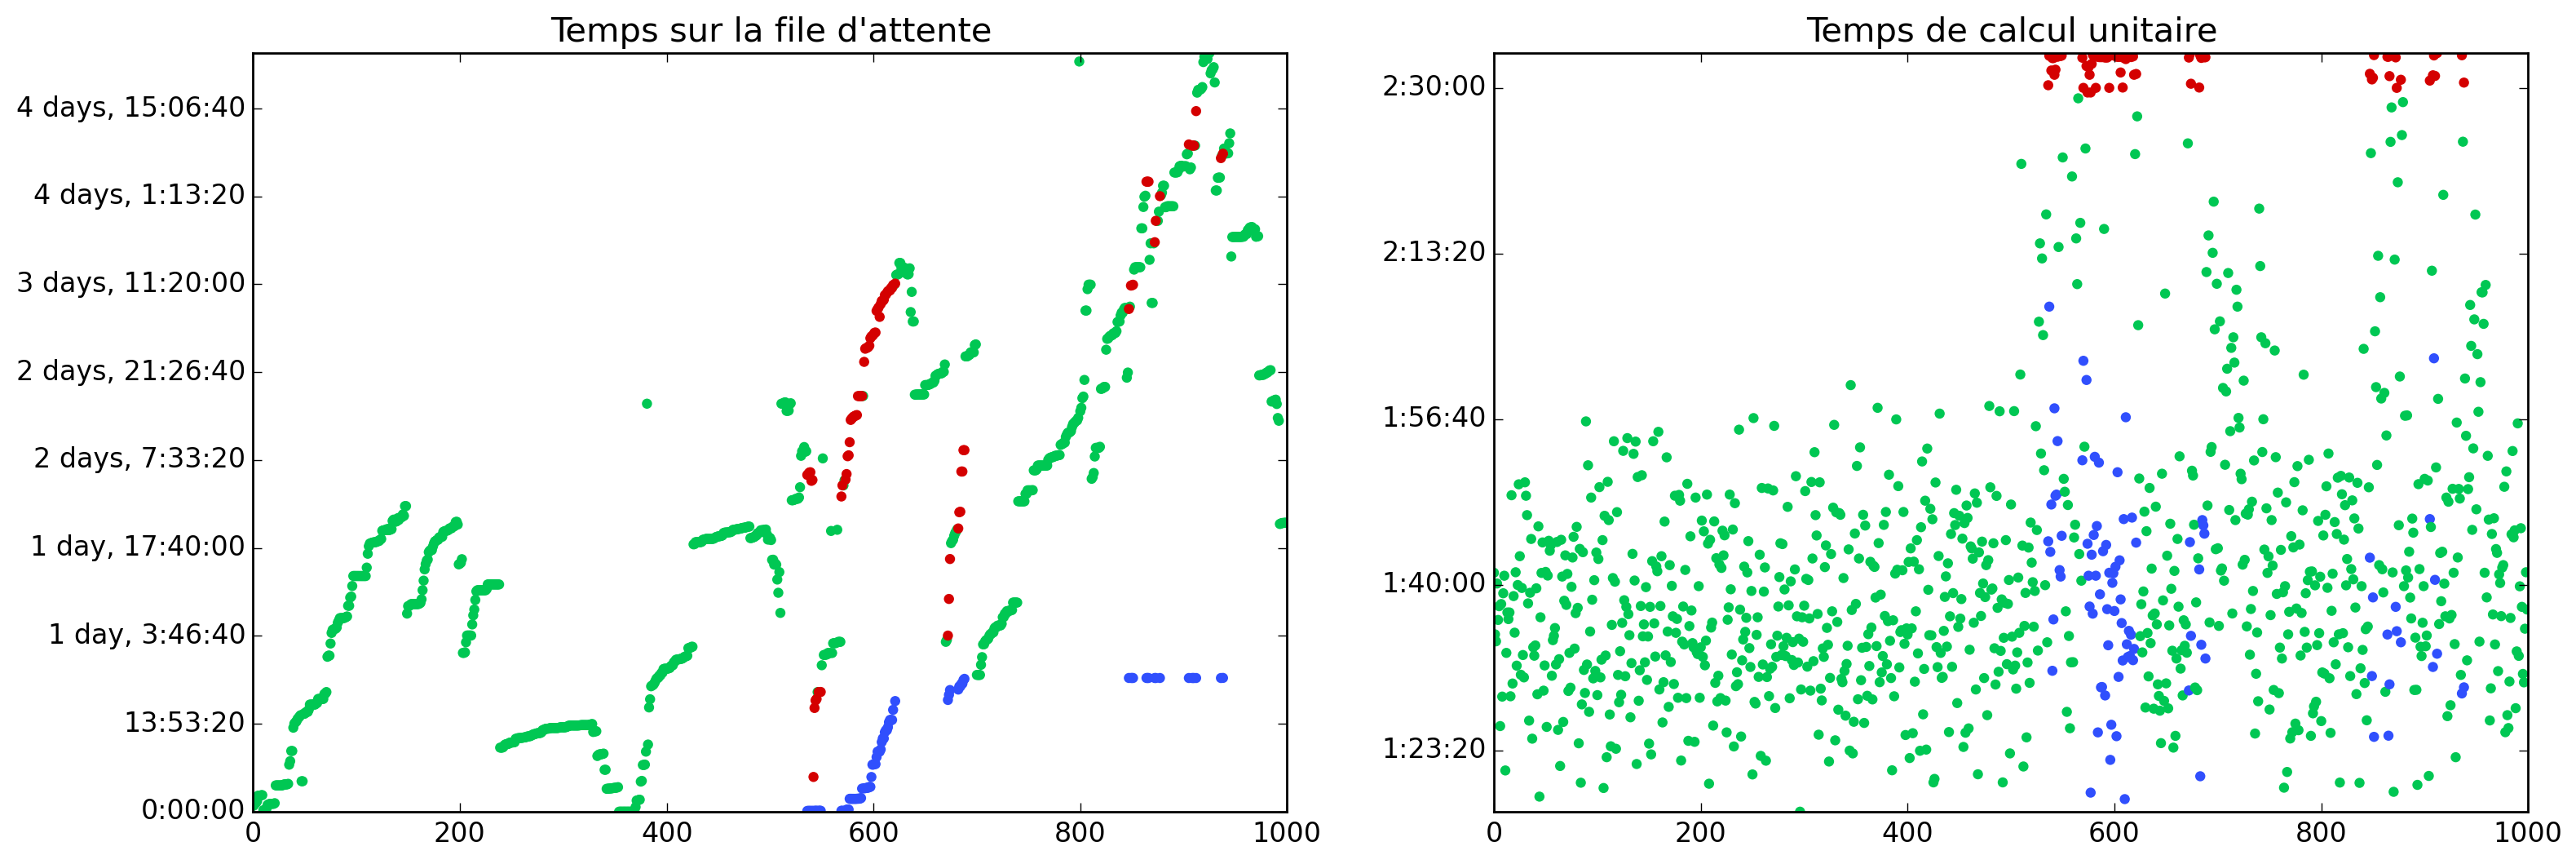
\includegraphics[width=0.9\textwidth]{./figure/Temps_DOE_Sobol_1000-white.png}
\end{frame}


\begin{frame}[fragile]
\frametitle{Parse output parameters 1/2}
\begin{itemize}
\item Common practice among scientific code is to create output files with
  the results of the simulation.
\item The output should then be parsed in order to get the output
  parameters of interest.
\item If it is a \texttt{.csv} file
\begin{itemize}
    \item \href{http://pandas.pydata.org/pandas-docs/stable/generated/pandas.read_csv.html}{pandas.read\_csv} is the fastest option, but it introduces pandas as a dependency.
    \item if speed is not an issue, try \href{http://doc.openturns.org/openturns-latest/sphinx/user_manual/_generated/openturns.coupling_tools.get_value.html}{ot.coupling\_tools.get\_value}, 
    \item or \href{http://docs.scipy.org/doc/numpy-1.10.0/reference/generated/numpy.loadtxt.html}{numpy.loadttxt}.
\end{itemize}
\end{itemize}
\end{frame}

\begin{frame}[fragile]
\frametitle{Parse output parameters 2/2}
\begin{itemize}
\item For \texttt{.xml} files \href{https://docs.python.org/2/library/xml.dom.minidom.html}{minidom} package from the python standard library does the trick.
\item If by any chance the external code returns the output parameters of
  interest to STDOUT, set \texttt{get\_stdout=True} when calling
  \texttt{ot.coupling\_tools.execute(...)}.  (or use \href{https://docs.python.org/2/library/subprocess.html#subprocess.check_output}{subprocess.check\_output})
\item For standard binary formats, there are python interfaces to \href{https://github.com/Unidata/netcdf4-python}{netcdf}
  and \href{http://www.h5py.org/}{HDF5}.
\item Otherwise, be creative and pythonic !
\end{itemize}
\begin{Verbatim}[xleftmargin=10mm]
def _parse_output(self):
    # Retrieve output (see also )
    xmldoc = minidom.parse('outputs.xml')
    itemlist = xmldoc.getElementsByTagName('outputs')
    Y = float(itemlist[0].attributes['Y1'].value)

    return [Y]
\end{Verbatim}
\end{frame}


\section{In use tools}
\label{sec-4}
\begin{frame}[fragile]
\frametitle{Managing data backups}
\begin{itemize}
\item Uncertainty studies tend to be expensive in computational time, it is then in your best interest to backup your simulation results !
\item \texttt{otwrapy} has two useful functions to do so:  \href{http://openturns.github.io/otwrapy/master/_generated/otwrapy.dump_array.html}{otwrapy.dump\_array} and  \href{http://openturns.github.io/otwrapy/master/_generated/otwrapy.load_array.html}{otwrapy.load\_array}
\item They are faster than a simple pickle.dump and pickle.load (because they use \texttt{protocol=2})
\item They offer the possibility to compress data with the \texttt{gzip} library. If the extension is \texttt{`pklz`}, it compresses by default.
\item Advice: Convert your \texttt{ot.Sample} to a \texttt{np.array} before dumping. An \texttt{np.array} is lighter !
\item Example: dump and compress
\end{itemize}
\begin{Verbatim}[xleftmargin=10mm]
import otwrapy as otw
otw.dump_array(np.array(X), 'InputSample.pklz', compress=True)
\end{Verbatim}

\begin{itemize}
\item ... and load
\end{itemize}
\begin{Verbatim}[xleftmargin=10mm]
import otwrapy as otw
import openturns as ot
X = otw.load_array('InputSample.pklz')
X = ot.Sample(X)
\end{Verbatim}
\end{frame}

\begin{frame}[fragile]
\frametitle{Catch exceptions when your code fails}
\begin{itemize}
\item In order to catch exceptions use the decorator \href{http://openturns.github.io/otwrapy/master/_generated/otwrapy.Debug.html}{otwrapy.Debug()} !
\item It encloses what happens inside a function into a try/catch
  structure and logs Exceptions when they are raised.
\item Useful when your wrapper is not used on an interactive
  environment like IPython or a Jupyter notebook.
\end{itemize}
\begin{Verbatim}[xleftmargin=10mm]
import otwrapy as otw
class Wrapper(ot.OpenTURNSPythonFunction):
    @otw.Debug('wrapper.log')
    def _exec(self, X):
        #Do stuff
        return Y
\end{Verbatim}
\end{frame}

\begin{frame}[fragile]
\frametitle{Creating a CLI for your wrapper}
\begin{itemize}
\item A command line interface allows you to run your wrapper in detached
  mode, e.g., through submission scripts on HPC clusters.
\item The \href{https://docs.python.org/3/library/argparse.html}{argparse} library might seem complicated, but they have a great
  cookbook and there are good chances that a simple copy/paste will be
  enough.
\item Take a look at the \href{https://github.com/openturns/otwrapy/tree/master/otwrapy/examples/beam}{beam wrapper}  for an example of a CLI interface
\end{itemize}
\begin{Verbatim}[xleftmargin=10mm]
if __name__ == '__main__':
    import argparse
    parser = argparse.ArgumentParser(description="Python wrapper example.")
    parser.add_argument('-X', nargs=3, metavar=('X1', 'X2', 'X3'),
        help='Vector on which the model will be evaluated')
    args = parser.parse_args()

    model = Wrapper(3, 1)
    X = ot.NumericalPoint([float(x) for x in args.X])
    Y = model(X)
    dump_array(X, 'InputSample.pkl')
    dump_array(Y, 'OutputSample.pkl')
\end{Verbatim}
\begin{itemize}
\item You can then execute your code from the command line :
\end{itemize}
\begin{Verbatim}[xleftmargin=10mm]
python wrapper.py –X 170 3 0.05
\end{Verbatim}
\end{frame}

\section{Parallelization}
\label{sec-7}
\begin{frame}[fragile]
\frametitle{Parallelizing the wrapper}
\begin{itemize}
\item Uncertainty studies fall into what we call \textit{embarrassingly parallel} (or \textit{pleasantly parallel}) patterns --> Repeat similar non communicating tasks over and over.
\item Good news, this means that they are very simple to parallelize.
\item But don't bother\ldots{} just let the magic happen with \href{http://openturns.github.io/otwrapy/master/_generated/otwrapy.Parallelizer.html}{otwrapy.Parallelizer()} !!
\end{itemize}
\begin{Verbatim}[xleftmargin=10mm]
import otwrapy as otw
from otwrapy.examples.beam import Wrapper
parallelized_beam_wrapper = otw.Parallelizer(Wrapper())
\end{Verbatim}
\end{frame}


\begin{frame}
\frametitle{Distributing calls on clusters or the cloud}
\begin{itemize}
\item But what if you want to distribute your wrapper calls on the cloud or
  on a cluster ?
\item otw.Parallelizer is no longer the way to go, for the moment\ldots{}
\item You can manage to make an heterogeneous office cluster with \href{http://ipyparallel.readthedocs.io/en/latest/}{IPyparallel} or \href{http://dispy.sourceforge.net/}{dispy}
\item For clusters and the cloud, rely on a good CLI interface of your
  wrapper and distribute your calls through submission scripts or
  cloud APIs (e.g., \href{https://www.simulagora.com/}{Simulagora} or \href{https://www.dominodatalab.com/}{Domino})
\end{itemize}
\end{frame}


\section{Conclusion}
\label{sec-8}
\begin{frame}
\frametitle{Conclusion}
\begin{itemize}
\item Take away message : Making a wrapper is all about preparing the
  input, executing the code and parsing the output on isolated working
  directories. Don't forget, in a multi-core era you don't have a
  choice, make your wrapper distributed !
\item By creating a CLI of your wrapper, you can easily distribute your
  calls on a cluster or on cloud platforms.
\item It is important to protect your wrapper with otw.Debug() so that
  you can have a traceback of raised Exceptions.
\item \href{http://doc.openturns.org/openturns-latest/sphinx/user_manual/_generated/openturns.PythonFunction.html}{ot.PythonFunction()} is a simpler alternative to
  \href{http://doc.openturns.org/openturns-latest/sphinx/user_manual/_generated/openturns.OpenTURNSPythonFunction.html}{ot.OpenTURNSPythonFunction()}, but you loose the ability to parameterize your wrapper when instantiating it.
\item \href{http://openturns.github.io/otwrapy/master/index.html}{otwrapy} is here for you ! Use it to avoid code boilerplate or as a simple cookbook.
\end{itemize}
\end{frame}


\begin{frame}
\frametitle{Thank you for your attention}

\begin{center}

\includegraphics[width=0.15\textwidth]{./figure/LogoPhiHaut-white.png}
\vfill
Gaëtan Blondet
\vfill
\href{mailto:blondet@phimeca.com}{blondet@phimeca.com}
\vfill
Github : \href{http://openturns.github.io/otwrapy/master/index.html}{otwrapy}
\end{center}
\end{frame}

\end{document}
